\documentclass[a4paper ]{article}

\usepackage{etex}		% clash when too many dimensions
\usepackage{lettrine}	% für ersten Buchstaben groß

\usepackage[english]{babel}
\usepackage[utf8x]{inputenc}
\usepackage{amsmath}
\usepackage{graphicx}
\graphicspath{{/Users/marcfabel/Dropbox/Uni/Tinbergen/MPhil/STATA/GRAPHS/}}
%\usepackage[colorinlistoftodos]{todonotes}
\usepackage{ amssymb }
\usepackage{amsmath}
\usepackage{parskip}
\setlength{\parindent}{0pt}
\DeclareGraphicsExtensions{.pdf,.png,.jpg}
\usepackage{booktabs}
\usepackage{longtable}
\usepackage{enumerate} % roman enumeration
\usepackage{wrapfig}

\usepackage[labelfont=bf,labelsep = period, singlelinecheck=off,justification=raggedright]{caption}%both together help to have subfigures, other specifications which are nice: labelformat = parens -> number in paranthesis
\usepackage[singlelinecheck=on]{subcaption}

%\usepackage{tikz}
%\usetikzlibrary{decorations.pathreplacing}

\usepackage[authoryear, round, comma]{natbib}

\usepackage{titlesec} %section headers 
\titleformat*{\section}{\large\bfseries}



\usepackage{dsfont} %Double stroke, e.g. for indicator function


\usepackage{afterpage}
\usepackage{lscape}
\usepackage{multirow}
\usepackage{adjustbox}

\usepackage[hyphens]{url}



\usepackage[usenames,dvipsnames,svgnames,table]{xcolor}
\definecolor{darkblue}{rgb}{0.0,0.0,0.6}

 \usepackage{hyperref}
 \hypersetup{
      colorlinks   = true,
     citecolor    = darkblue,
 	linkcolor= darkblue,
     urlcolor=darkblue }

\usepackage[
	top    = 2.3cm,
	bottom = 2cm,
	left   = 1.8cm,
	right  = 1.8cm]{geometry}		%option: showframe=true (see page boundaries)
	
\usepackage{changepage} % adjust width on sides of the page, needed tto place tables in the middle of the page





\usepackage{pdflscape}
\usepackage{layouts}% temporär, zurbestimmung von textwdith





%\makeatletter
%\def\input@path{{tables/KKH/}}
%%or: \def\input@path{{/path/to/folder/}{/path/to/other/folder/}}
%\makeatother

\graphicspath{{../../analysis/graphs/population/}}

\usepackage{supertabular}
\author{Marc Fabel}
\title{Comparisson of population concepts}
\date{Last revision of this document: \today} 
\begin{document}
\maketitle
This document will compare our different population concepts: 
\begin{enumerate}
\item True number of births (Destatis)
\item The approximation (MZ weights + Regionalstatistik)
\item Same with aggregation over Kreise
\end{enumerate}

\bigskip
Notes to the figures:
\begin{itemize}
\item The blue range depicts the range of the approximated population numbers over the different survey years (2005-2013). This is our "standard" specification (what we sent to Janisch).
\item The grey range is almost the same. Instead of collapsing over the Kreise (without correction), I collapse over the Länder (did so in the local analysis now)
\item The red dot indicates the number of births (destatis) in the respective month of birth. 
\end{itemize}

%*************************************************************
%REFORM 1:
\begin{figure}[h]
\centering
\caption{Reform 1: 1976 - 1980}
\begin{subfigure}[t]{0.48\textwidth}
		\centering
		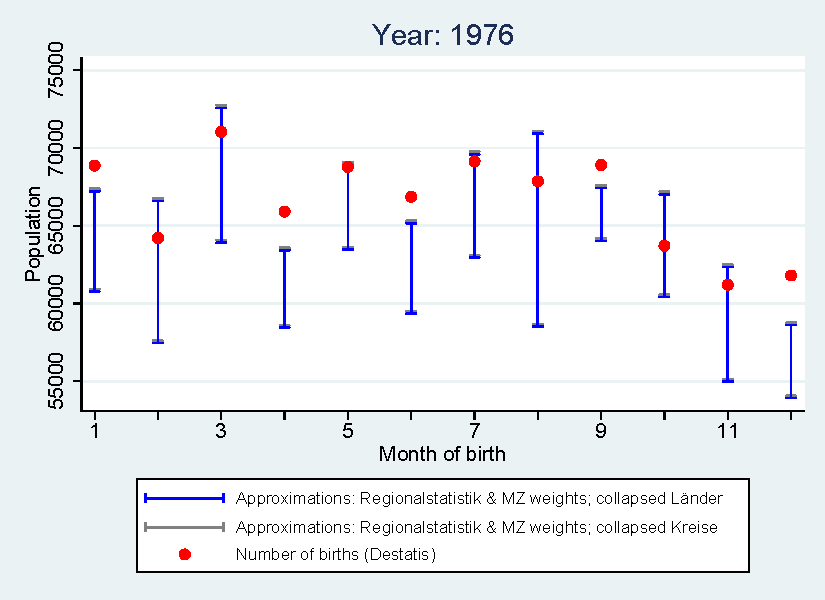
\includegraphics[width=0.99\textwidth]{comparison_population_1976.pdf}		
\end{subfigure}
\begin{subfigure}[t]{0.48\textwidth}
		\centering
		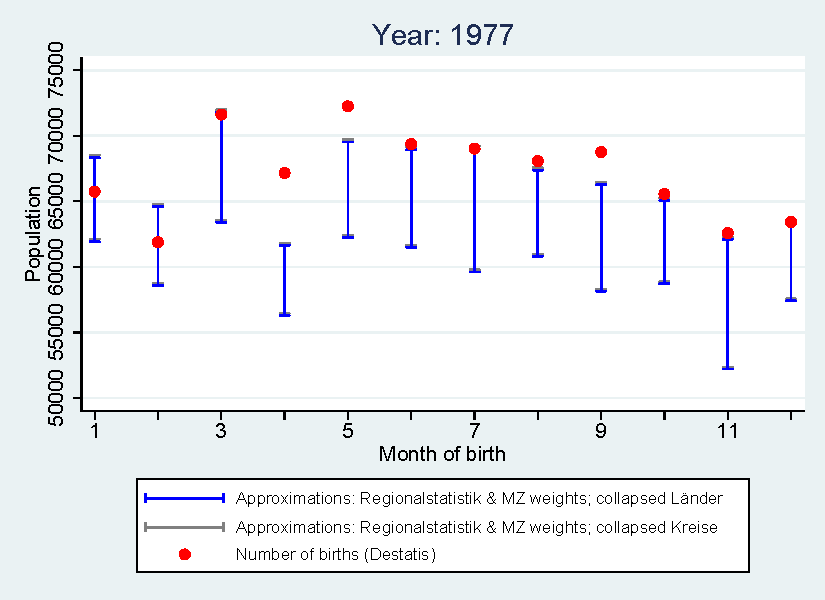
\includegraphics[width=0.99\textwidth]{comparison_population_1977.pdf}		
\end{subfigure}
\begin{subfigure}[t]{0.48\textwidth}
		\centering
		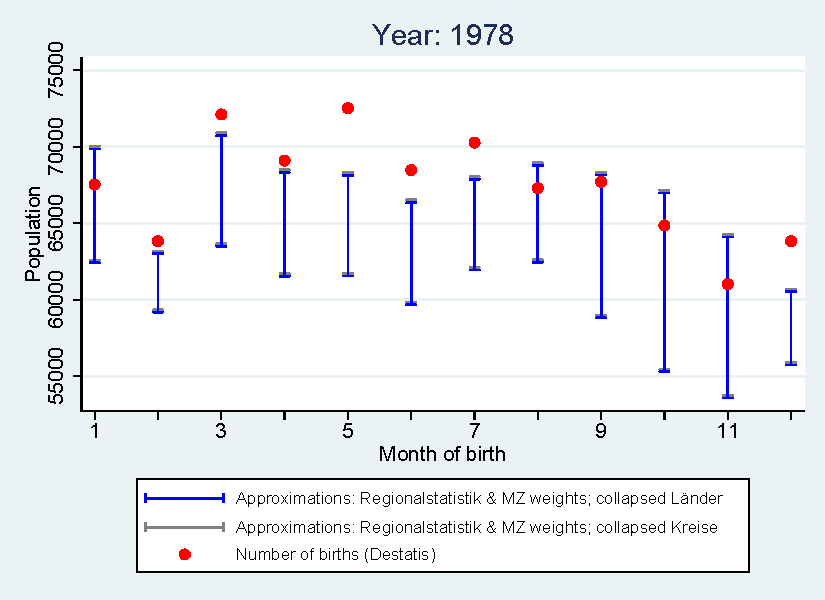
\includegraphics[width=0.99\textwidth]{comparison_population_1978.pdf}		
\end{subfigure}
\begin{subfigure}[t]{0.48\textwidth}
		\centering
		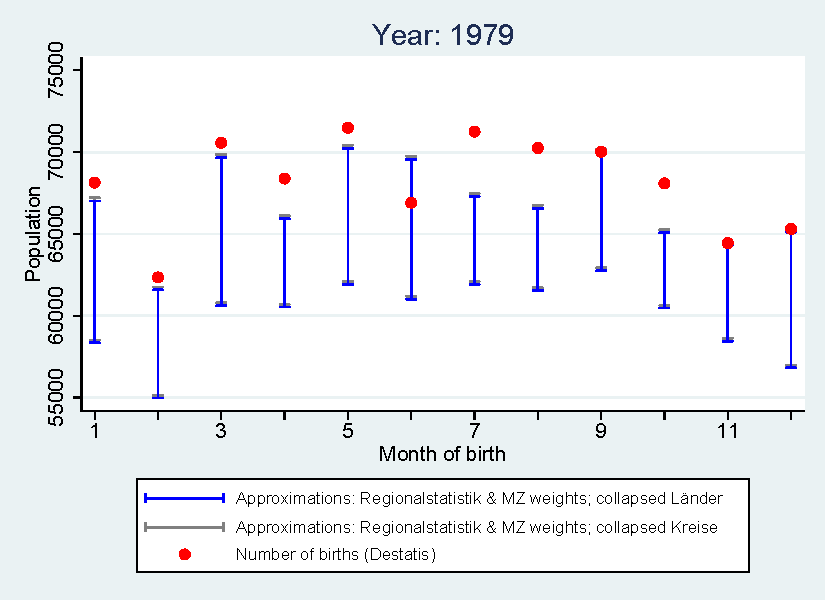
\includegraphics[width=0.99\textwidth]{comparison_population_1979.pdf}		
\end{subfigure}
\begin{subfigure}[t]{0.48\textwidth}
		\centering
		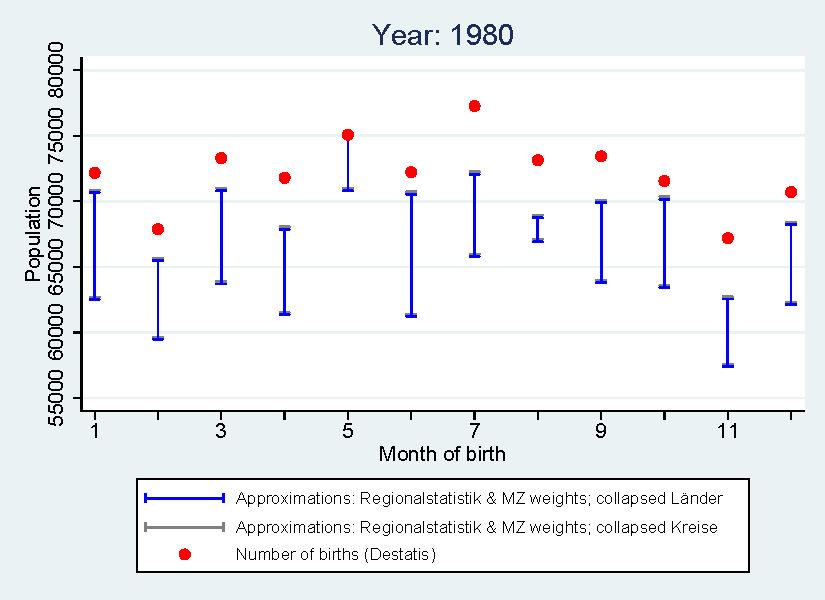
\includegraphics[width=0.99\textwidth]{comparison_population_1980.pdf}		
\end{subfigure}
\end{figure}
%*************************************************************
%REFORM 2:
\begin{figure}[h]
\centering
\caption{Reform 2: 1985 - 1989}
\begin{subfigure}[t]{0.48\textwidth}
		\centering
		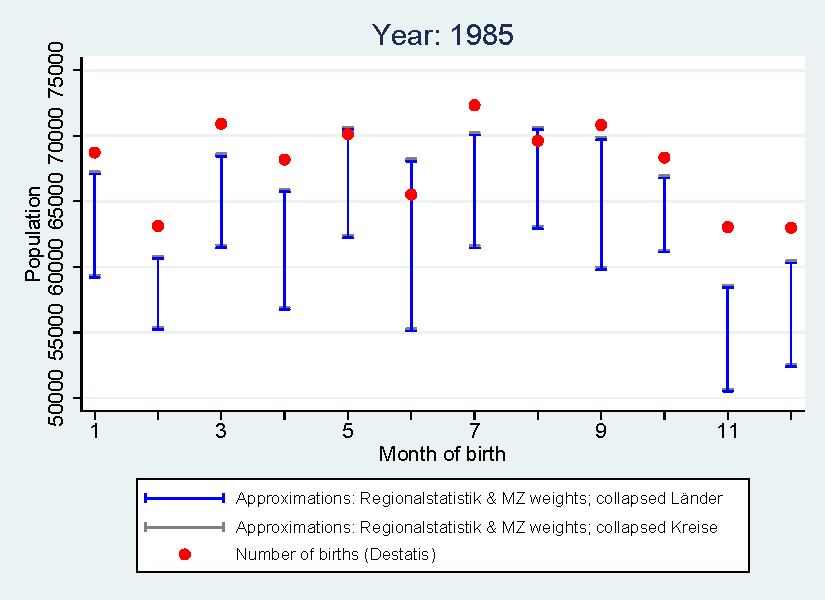
\includegraphics[width=0.99\textwidth]{comparison_population_1985.pdf}		
\end{subfigure}
\begin{subfigure}[t]{0.48\textwidth}
		\centering
		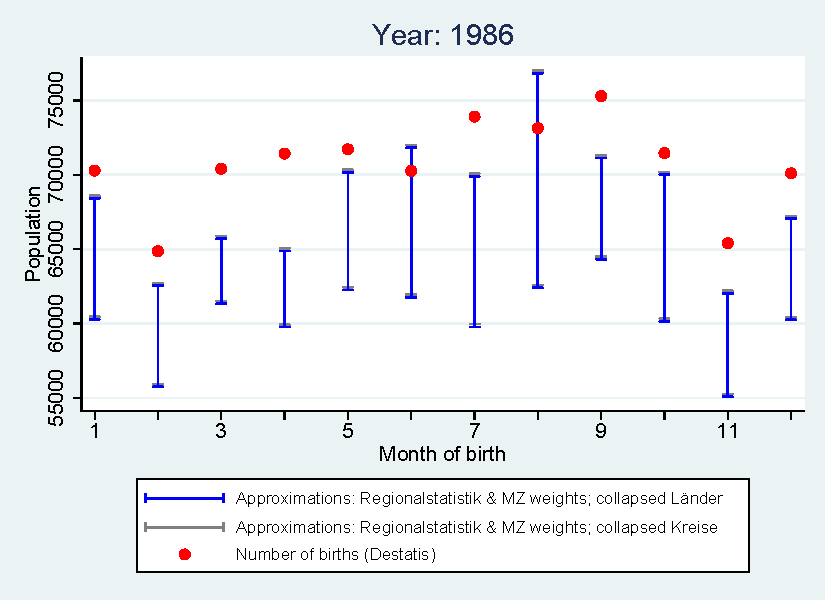
\includegraphics[width=0.99\textwidth]{comparison_population_1986.pdf}		
\end{subfigure}
\begin{subfigure}[t]{0.48\textwidth}
		\centering
		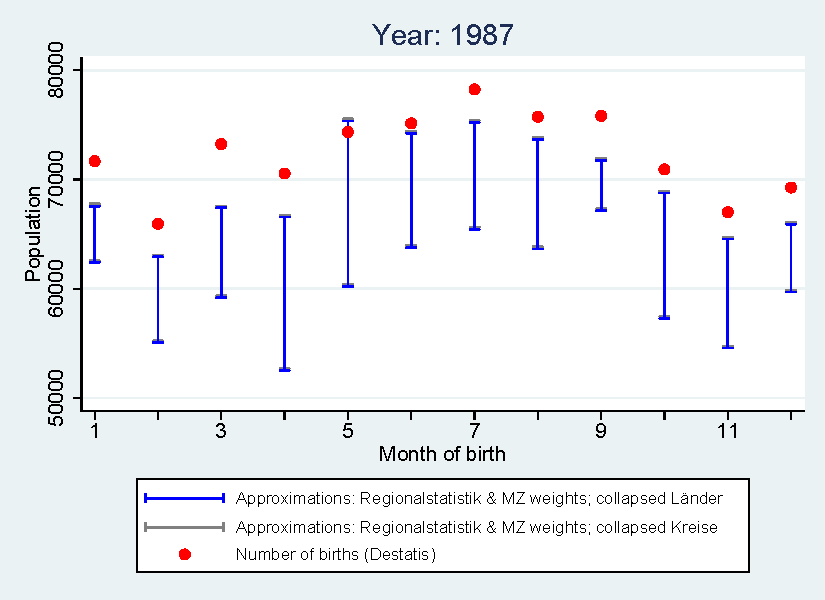
\includegraphics[width=0.99\textwidth]{comparison_population_1987.pdf}		
\end{subfigure}
\begin{subfigure}[t]{0.48\textwidth}
		\centering
		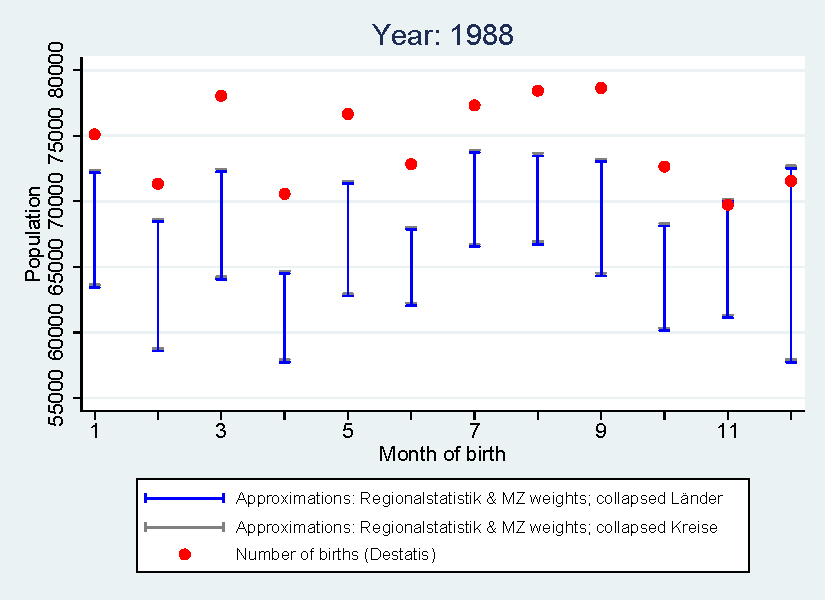
\includegraphics[width=0.99\textwidth]{comparison_population_1988.pdf}		
\end{subfigure}
\begin{subfigure}[t]{0.48\textwidth}
		\centering
		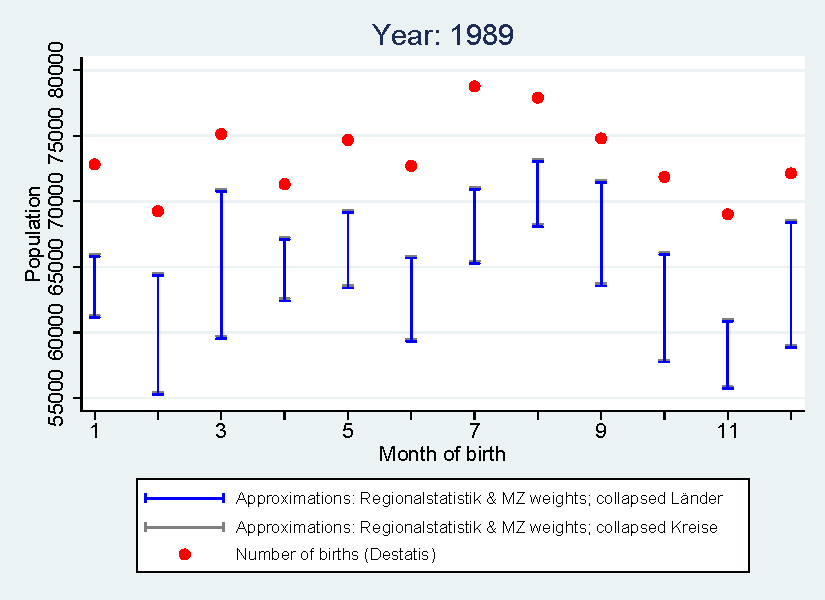
\includegraphics[width=0.99\textwidth]{comparison_population_1989.pdf}		
\end{subfigure}
\end{figure}
%*************************************************************
%REFORM 3:
\begin{figure}[h]
\centering
\caption{Reform 3: 1990 - 1995}
\begin{subfigure}[t]{0.48\textwidth}
		\centering
		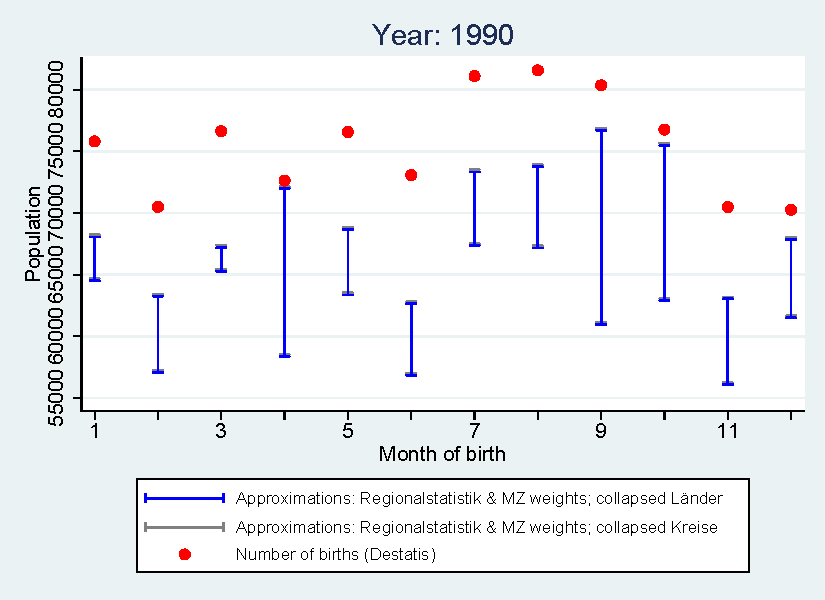
\includegraphics[width=0.99\textwidth]{comparison_population_1990.pdf}		
\end{subfigure}
\begin{subfigure}[t]{0.48\textwidth}
		\centering
		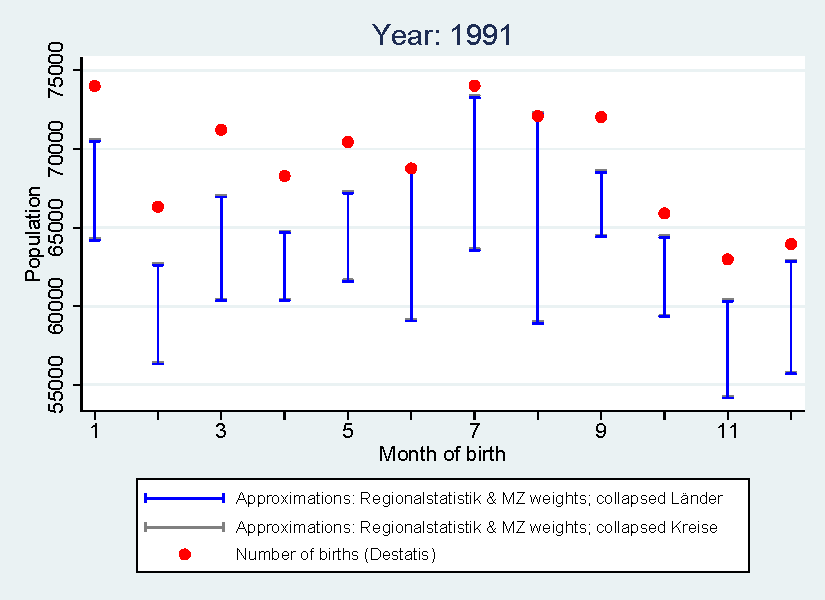
\includegraphics[width=0.99\textwidth]{comparison_population_1991.pdf}		
\end{subfigure}
\begin{subfigure}[t]{0.48\textwidth}
		\centering
		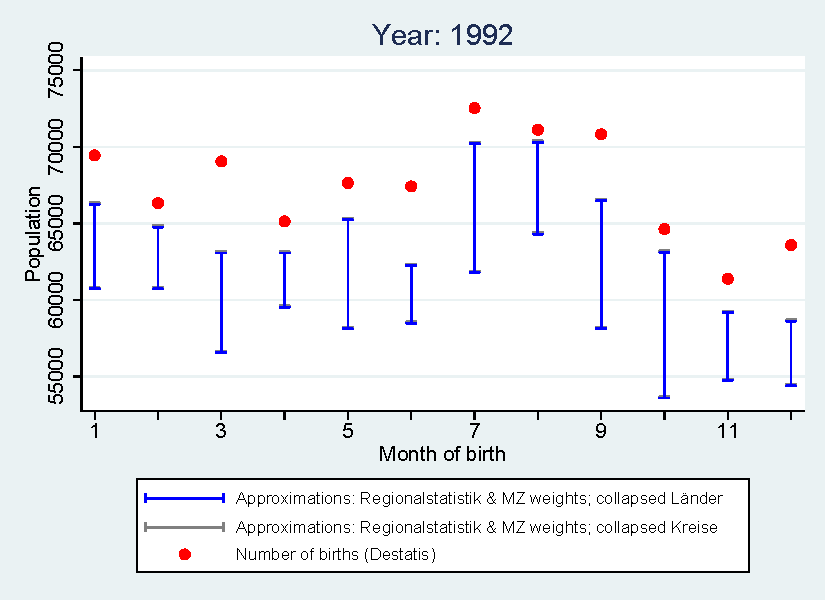
\includegraphics[width=0.99\textwidth]{comparison_population_1992.pdf}		
\end{subfigure}
\begin{subfigure}[t]{0.48\textwidth}
		\centering
		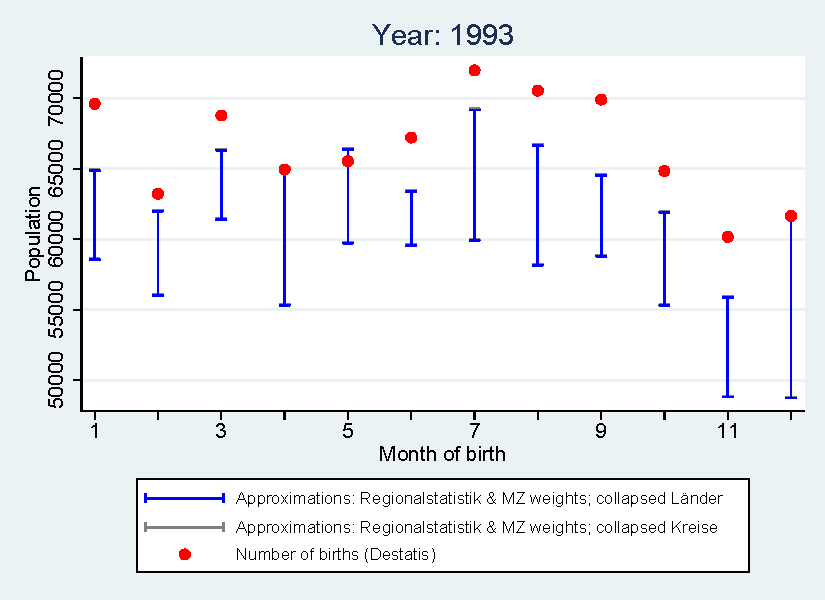
\includegraphics[width=0.99\textwidth]{comparison_population_1993.pdf}		
\end{subfigure}
\begin{subfigure}[t]{0.48\textwidth}
		\centering
		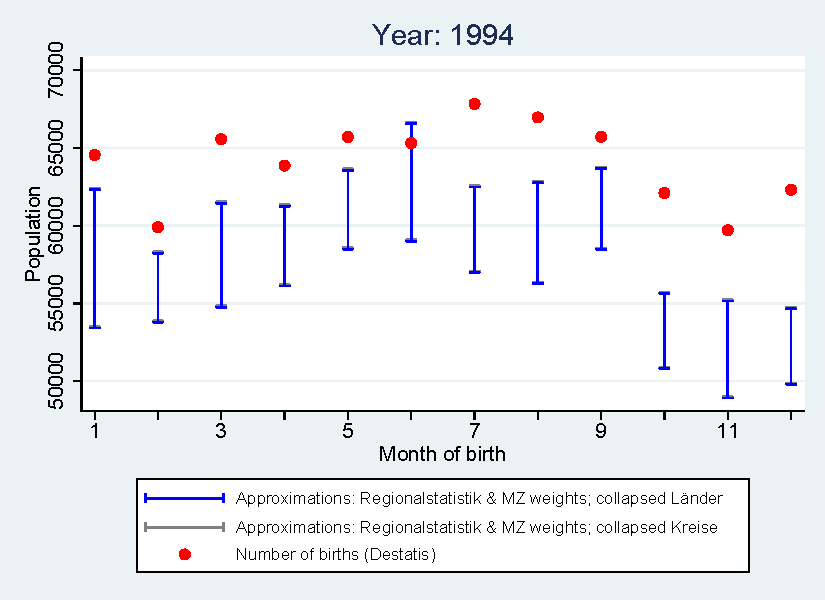
\includegraphics[width=0.99\textwidth]{comparison_population_1994.pdf}		
\end{subfigure}
\begin{subfigure}[t]{0.48\textwidth}
		\centering
		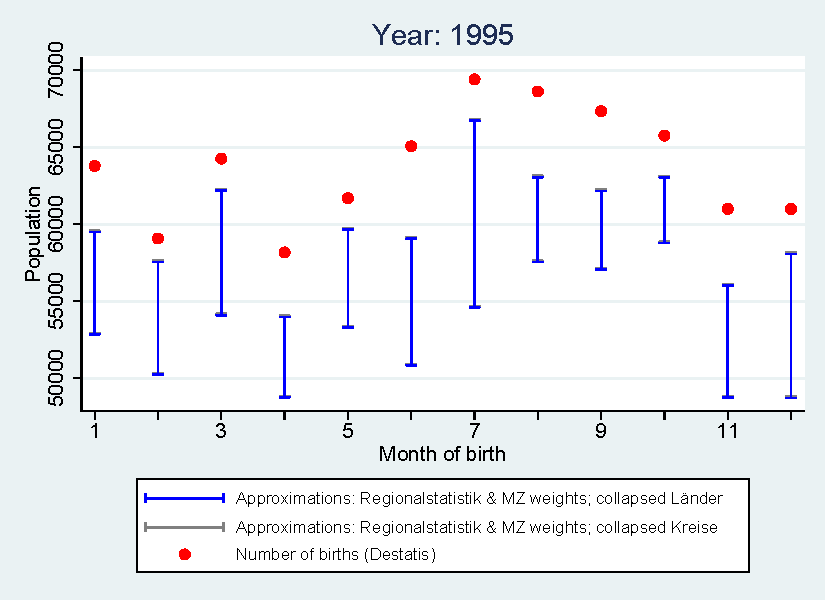
\includegraphics[width=0.99\textwidth]{comparison_population_1995.pdf}		
\end{subfigure}
\end{figure}



\end{document}